\label{c:Components}	
This chapter describes the hardware and software used in the experiments. An illustration of the final architecture can be found in \autoref{sec:architecture}.
  
\section{Hardware} \label{sec:Hardware}
\subsection{The High-speed Cameras and related Equipment}
The two cameras used in the scenario are color high-speed cameras of the model \textit{CR3000x2} (\textit{CamRecord} series) from \textit{Optronis}. 

The following list summarizes the model's specifications (a full data sheet is included in the digital appendix of this thesis):
\begin{itemize}
\item \textbf{Input and output interfaces (I/O-interfaces):}
 \begin{itemize}
  \item Gigabit-Ethernet (GigE)
  \item VGA video output
  \item Interfaces for external trigger, camera synchronization and low-voltage power supply (see \autoref{fig:camSpecs}a)
 \end{itemize}
\item \textbf{Mechanical interfaces:}
 \begin{itemize}
  \item Nikon F-Mount or C-Mount
  \item Screw threads for camera tripods etc. on three sides (\nicefrac{1}{4}-20 UNC), as seen in \autoref{fig:camSpecs}b 
 \end{itemize}  
\item \textbf{Sensor resolution:} 1696 x 1710 pixel
\item \textbf{Frame rate:} 540 fps (at max. sensor resolution)\footnote{The cameras can have higher frame rates with lower sensor resolutions.}
\end{itemize}

\begin{figure}[htbp]
		\centering
		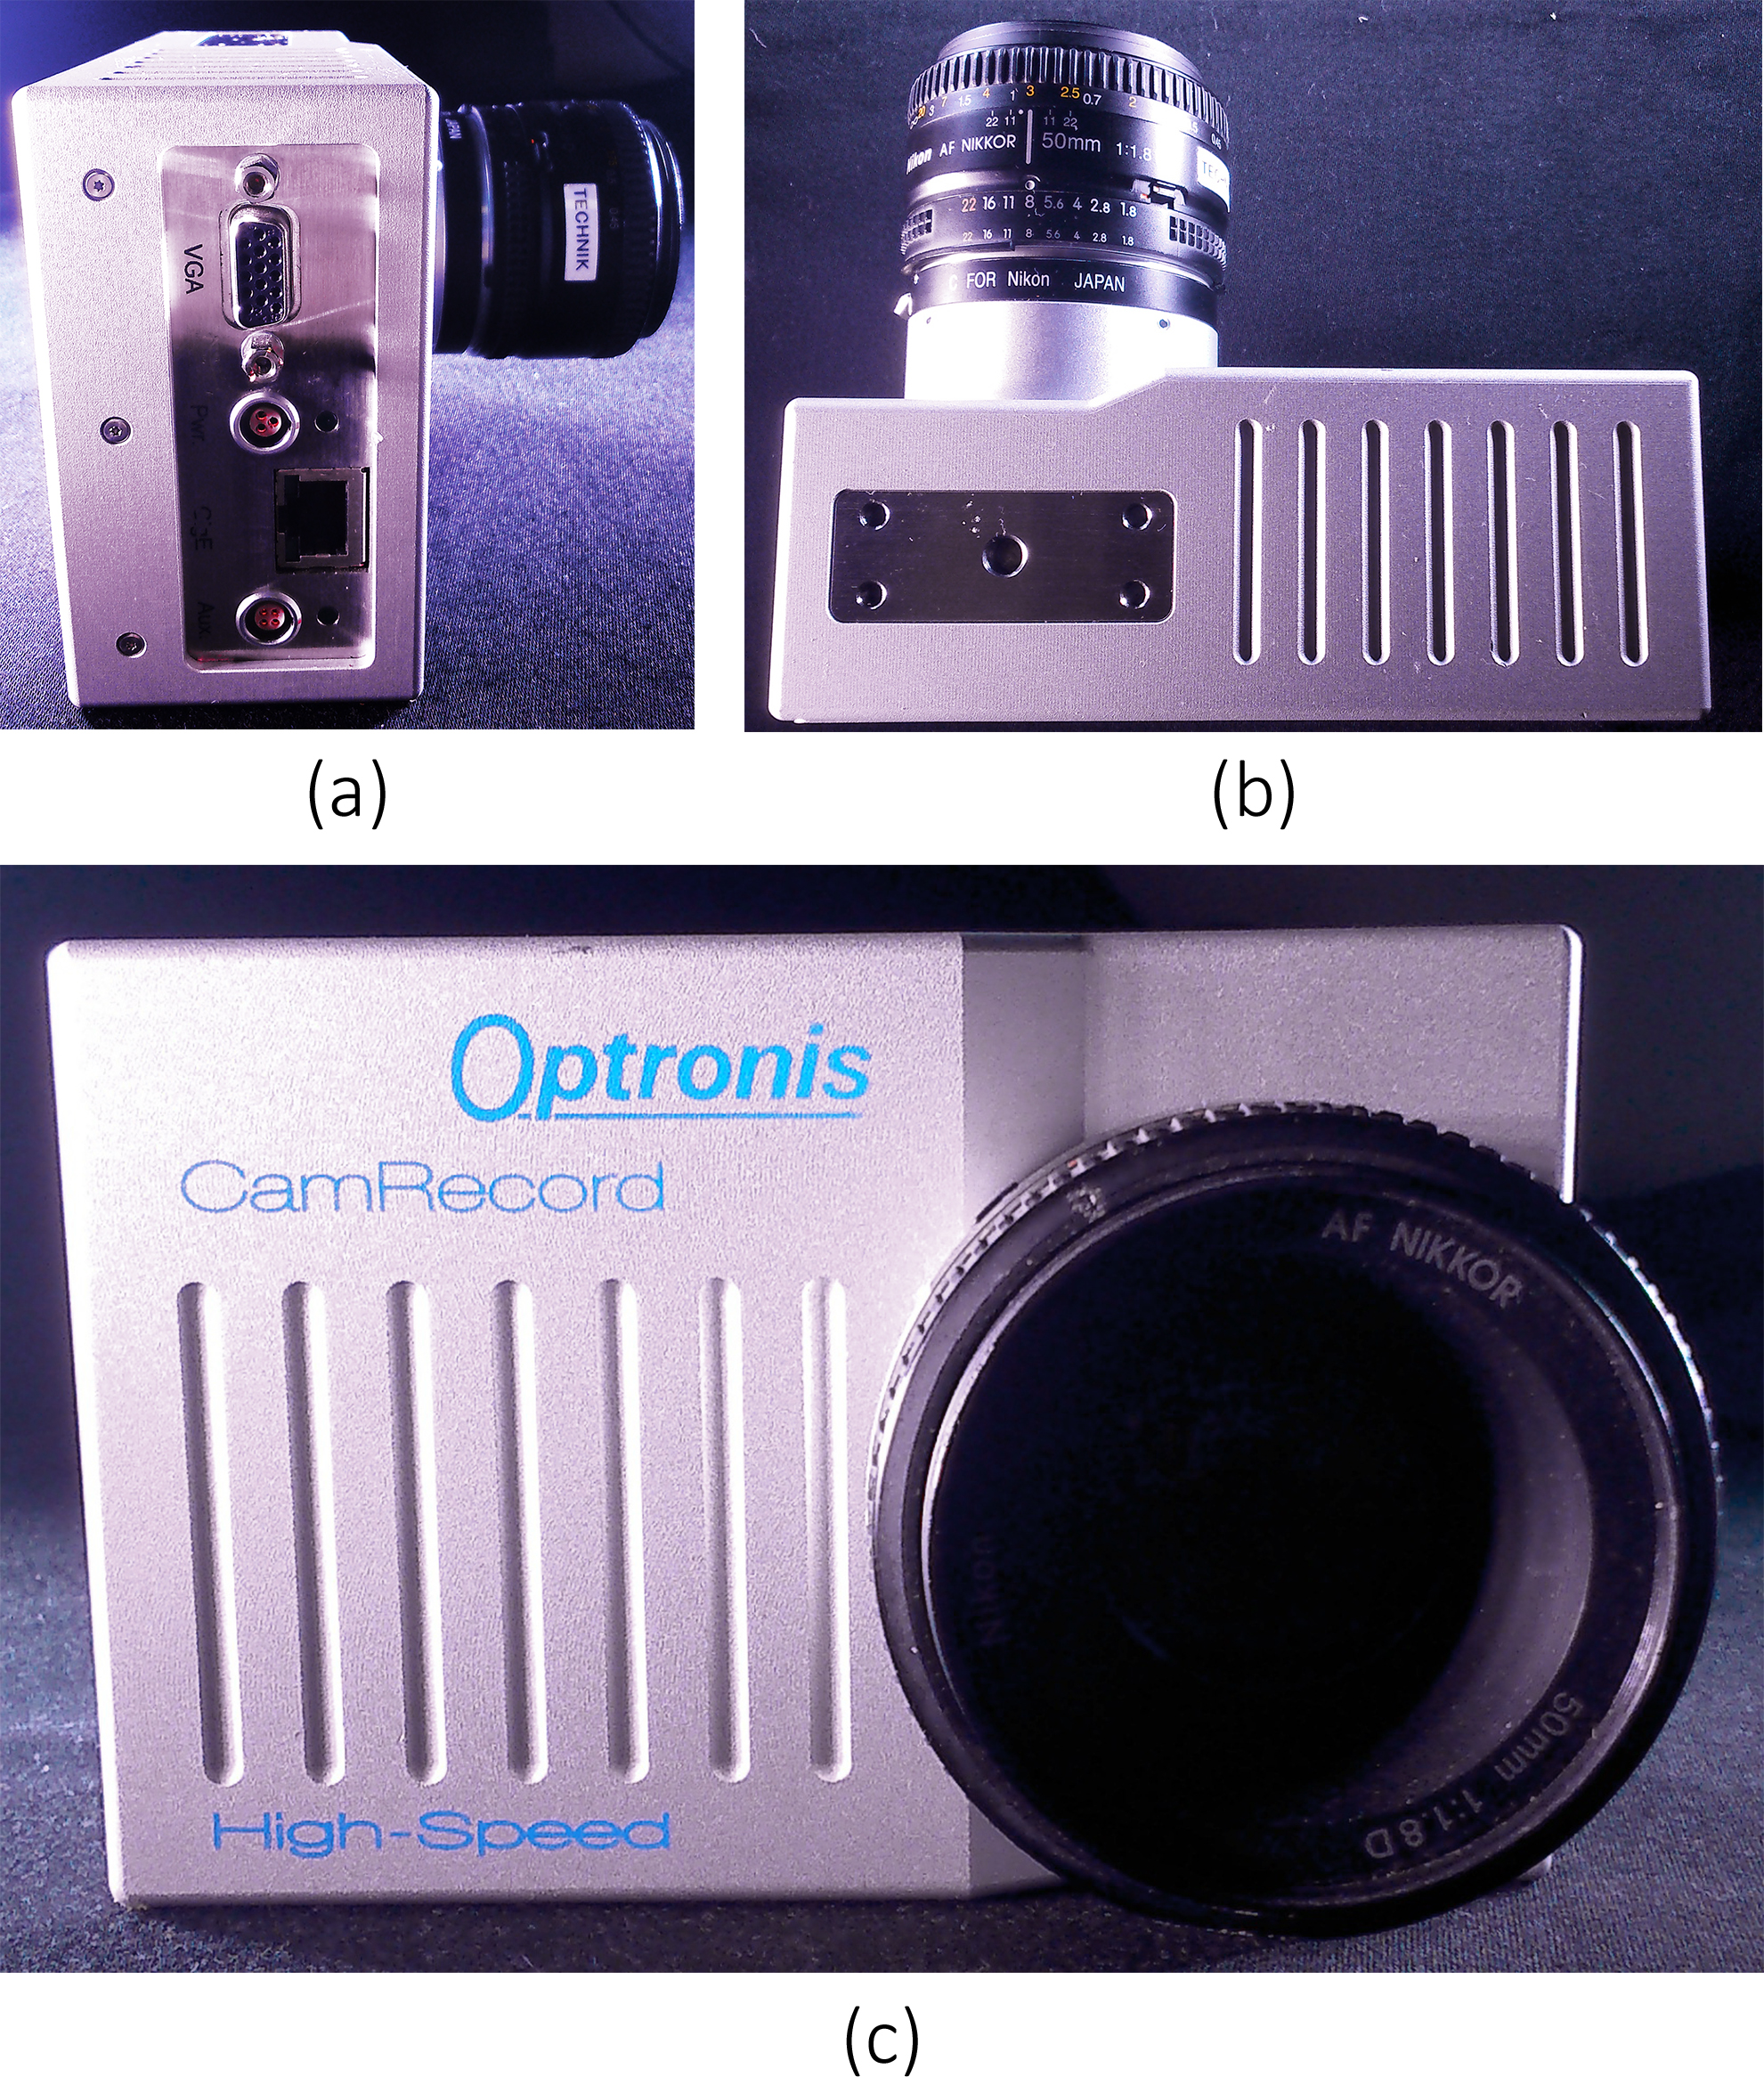
\includegraphics[width=0.8\textwidth]{figures/cameraSpecs}
		\caption[Camera from different angles]{The CR3000x2 high-speed camera from different angles: \textbf{(a)} I/O-interfaces at the side; \textbf{(b)} top view with one of the three screw threads; \textbf{(c)} frontal view.}
		\label{fig:camSpecs}
\end{figure}

The image sequences can be directly exported into the file formats BMP, TIFF, AVI or MPEG. Since the captured data uses a lot of storage, a sufficiently large hard disk is necessary.
In the following experiments the cameras will have this set-up (from the perspective of the cameras' viewing direction):

\paragraph{Right camera.}
CR3000x2 camera with the number \textit{1838-ST-C-013} and 8 GB ring buffer, set as synchronization master due to the smaller buffer size\footnote{The smaller buffer size serves as a benchmark for the overall capture duration since this camera could not store more footage.}.

\paragraph{Left camera}
CR3000x2 camera with the number \textit{1838-ST-C-013} and 16 GB ring buffer.

\paragraph{Lense.}
Two simple \textit{Nikon} 50 mm lenses with fixed focal lengths were used (see \autoref{fig:camSpecs}).

\paragraph{Cables and connections.}
To connect the cameras with each other, with the trigger (see below) and with the computer, the following data cables were used:
\begin{itemize}
\item Three \textit{cat 7 Ethernet cables}: for connecting the two cameras with the computer.
\item Three \textit{coaxial cables} with \textit{BNC connectors}: for the trigger and for the synchronization.
\end{itemize}
Furthermore a gigabit Ethernet switch is needed for the data transfer between the two cameras and the computer.

\paragraph{Synchronized triggering.}
The cameras can be triggered by software (see \autoref{ssec:Timebench}) or with a mechanical external trigger (see \autoref{fig:ExTrigger}). The latter was used in the final architecture. The external trigger and the two cameras are connected with two coaxial cables with \textit{BNC connectors}.  

\begin{figure}[htbp]
		\centering
		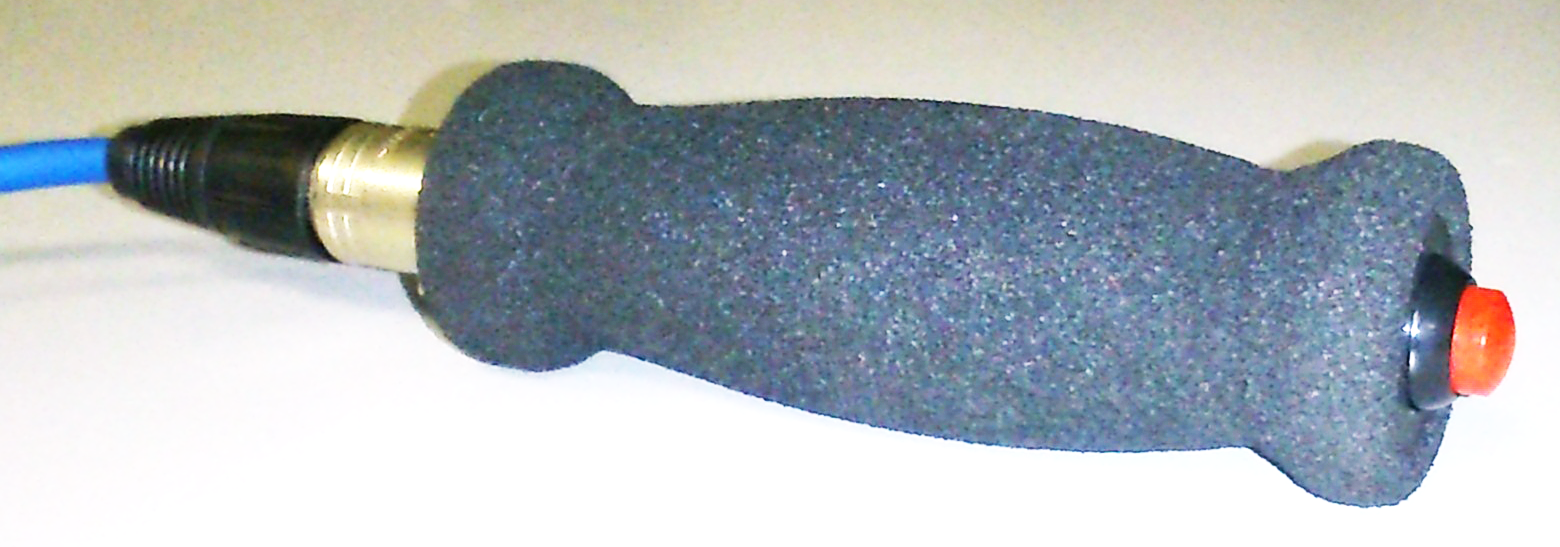
\includegraphics[width=0.8\textwidth]{figures/Trigger}
		\caption[External mechanical trigger]{External mechanical trigger.}
		\label{fig:ExTrigger}
\end{figure}

\paragraph{Lighting.}\label{par:Lighting}
The high frame rate of the cameras results in serious lighting issues. The scene has to be very brightly illuminated to get satisfying image results, which is especially true for a successful camera calibration. In addition, lighting must not be arbitrary, because the dim cycles of certain lamp filaments are visible as flicker on the images due to the high speed of the cameras. Another type of artifact can arise with the usage of \textit{HMI lighting}. With these lights the electrical arc traveling through the gas can be visible on the output images (called \textit{Arc Wander}\index{Arc Wander})\footnote{A nice summary of this topic can be found at \url{http://www.lovehighspeed.com/lighting-for-high-speed/}. The website states that a frame rate of 1000 fps needs 5.25 times more light than a frame rate of 25 fps.}. To avoid these problems, either lamps with constantly lit filaments or special LED lights need to be used. LED lights come in a variety of refresh rates and generally the ones designed for the film industry will not show any flicker as long as they are not dimmed. Hence, three \textit{EUROLITE} LED lights and one MultiLED from \textit{Optronis} were used to illuminate the scene. The final lighting set-up can be seen in \autoref{fig:Lighting}.

\begin{figure}[htbp]
		\centering
		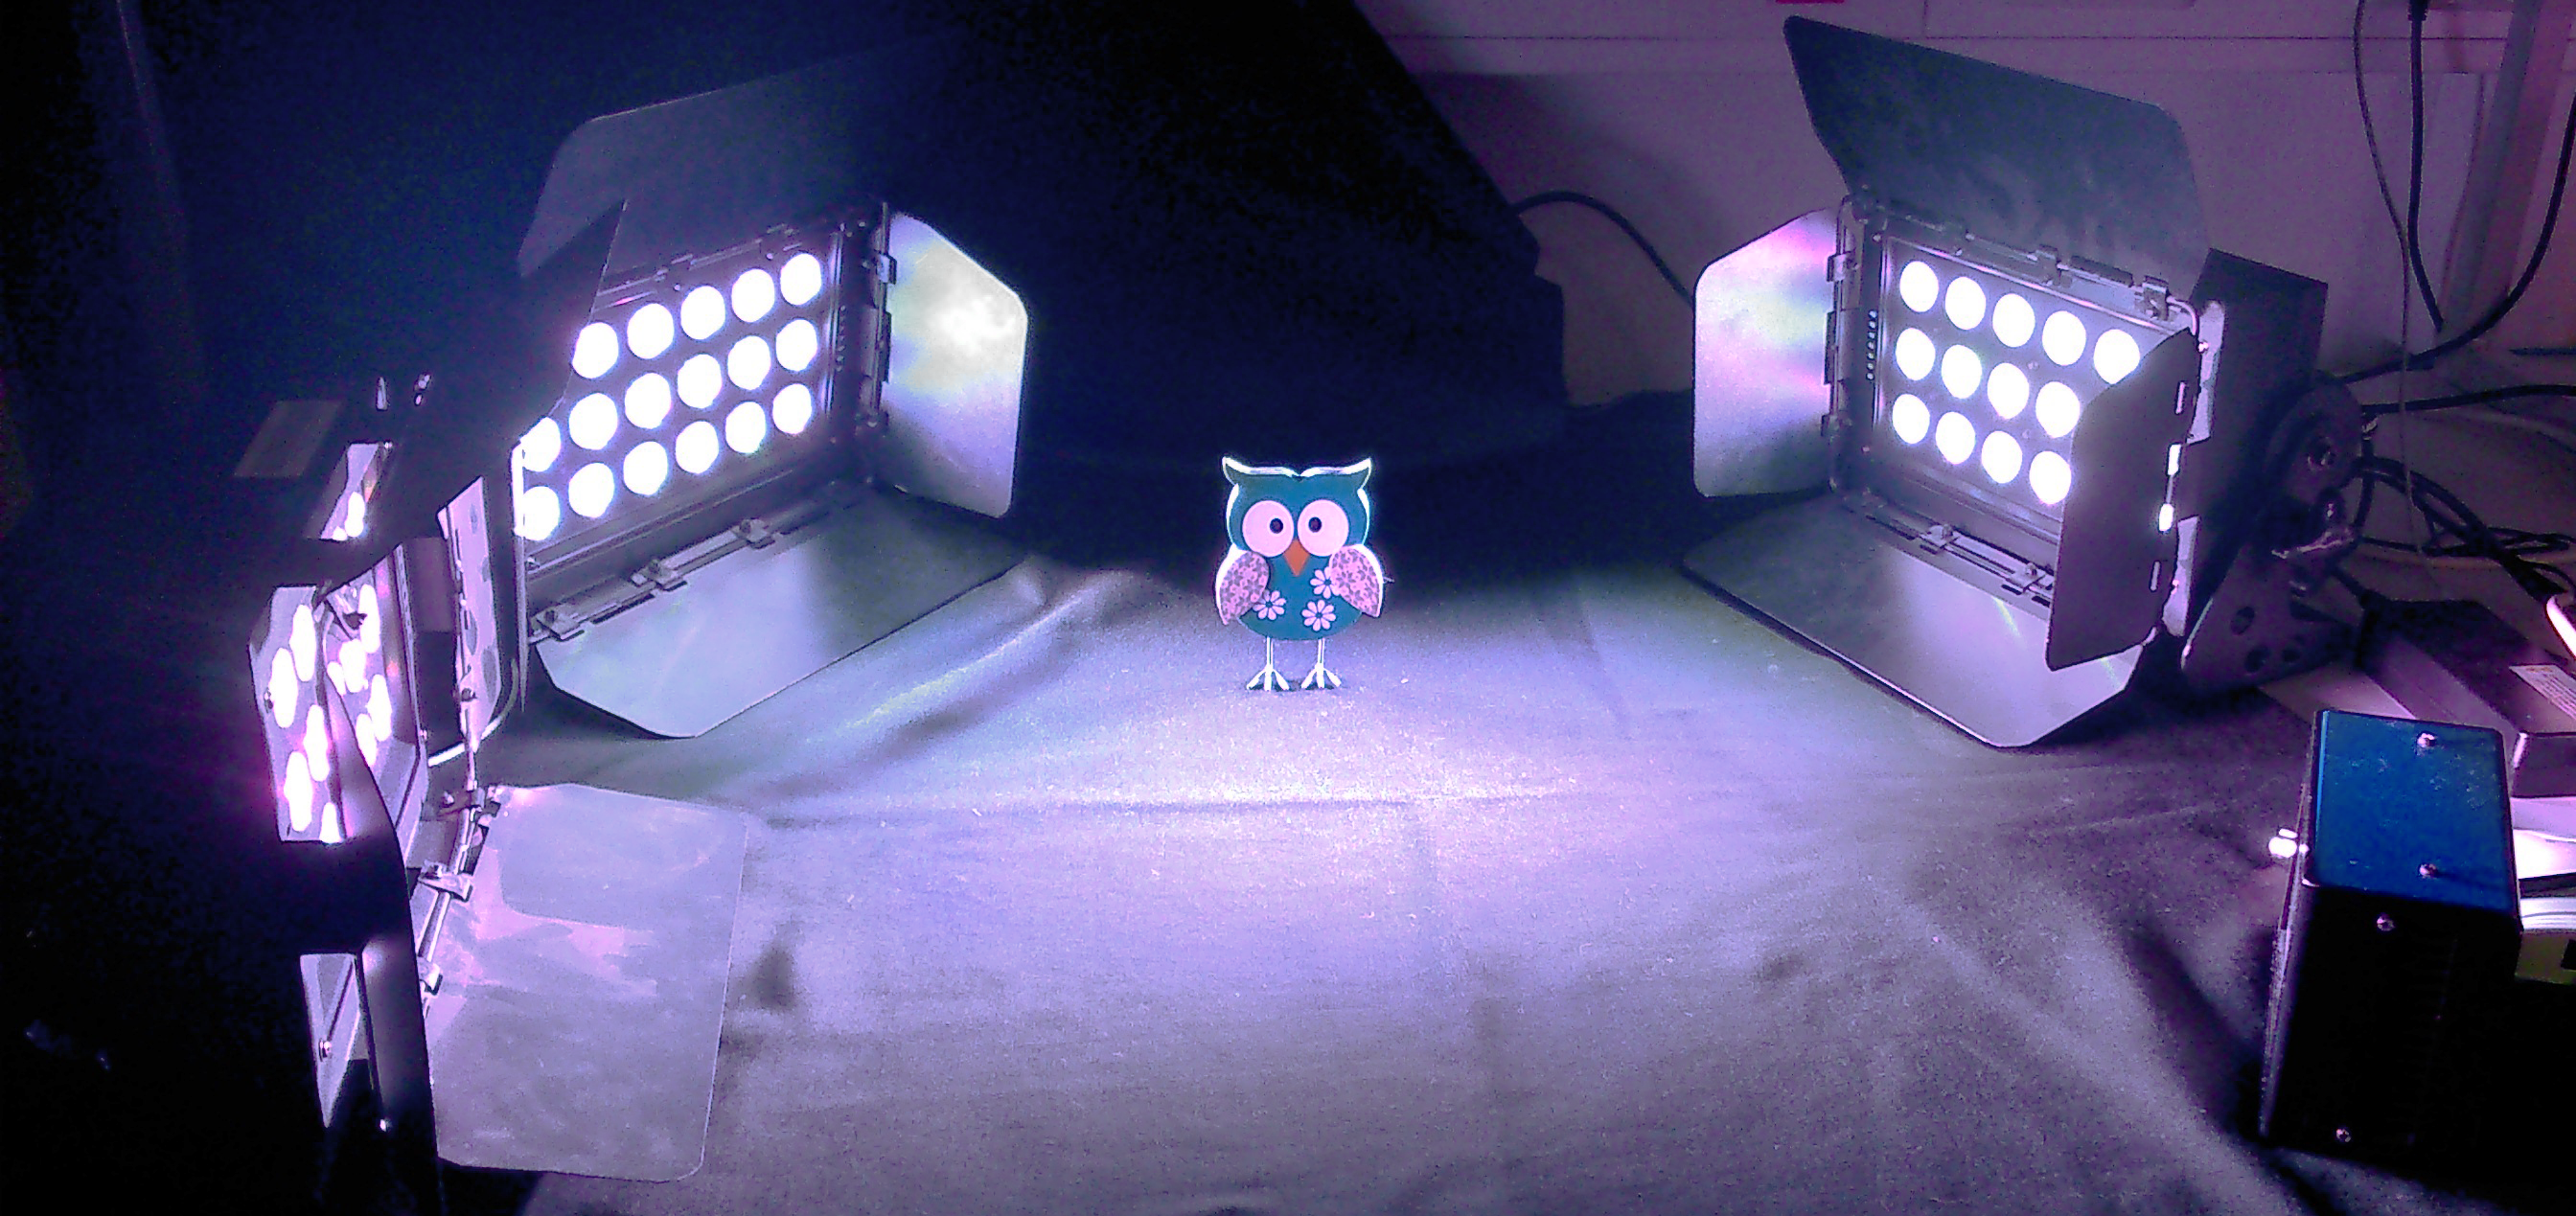
\includegraphics[width=0.8\textwidth]{figures/lighting}
		\caption[Lighting set-up]{Lighting set-up consisting of three \textit{EUROLITE LED CLS-18 QCL} and one MultiLED }
		\label{fig:Lighting}
\end{figure}

\subsection{Calibration Pattern}\label{ssec:calibPattern}
The stereo calibration toolbox for MATLAB (explained in \autoref{ssec:stereoCalibToolbox}) uses a checkerboard pattern to calibrate cameras. It does not natively support other calibration patterns. It is important to have an odd number of squares in one direction and an even number in the other direction, which lets the app determine the orientation of the pattern. The longer side will be the $x$-direction (\cite{StereoCalib.2016}).
A checkerboard pattern can be loaded directly in MATLAB with 

\begin{lstlisting}
open checkerboardPattern.pdf;
\end{lstlisting}

A simple pattern is included in the appendix of this thesis. The pattern needs to be printed out as clean as possible and needs to be affixed to a flat surface. In the first few experiments a checkerboard with a square size of 30 cm was used. Because the cameras' field of view is small (the reasons for this are explained in \autoref{c:Experiments}), the size of the checkerboard needed to be reduced. The final checkerboard pattern has a square size of 3 mm (as seen in \autoref{fig:smallCalibPattern}). The process of checkerboard recognition is explained in more detail in \autoref{sec:Calibration}.  

\begin{figure}[htbp]
		\centering
		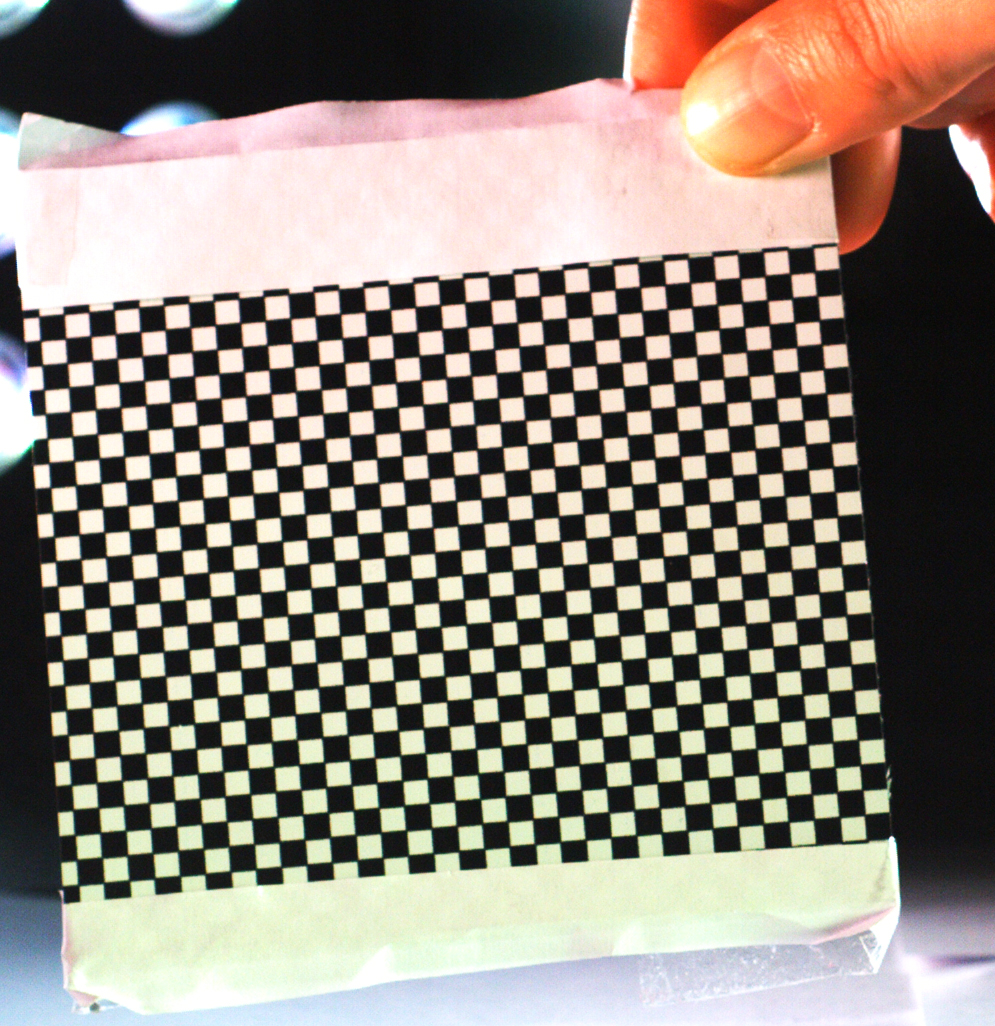
\includegraphics[width=0.5\textwidth]{figures/smallCalibPattern}
		\caption[Checkerboard pattern for camera calibration]{Checkerboard pattern with a square size of 3 mm for camera calibration}
		\label{fig:smallCalibPattern}
\end{figure}

\section{Software} \label{sec:Software}
This thesis was written in \LaTeX . Other software used is explained in the following sections.

\subsection{Timebench} \label{ssec:Timebench}
The software \textit{TimeBench}\footnote{More information about TimeBench can be found on the official website at \url{http://www.optronis.com/en/products/high-speed-cameras/software.html}.} was developed by \textit{Optronis} and is included in the delivery of their high-speed camera series. It lets the user capture high-speed image sequences and comes with several tools to adjust, analyze and export these sequences (\cite{Optronis.2016}). 

This software was chosen due to its close connection to the high-speed cameras that were used. It is also well optimized to process large amounts of image data. The software can also be used with third party video cameras.

TimeBench was first used to create image pair sequences of the calibration pattern in several positions and angles for the camera calibration process (see \autoref{sec:Calibration}). The software was then used to record a high-speed image sequence of moving objects, the objects were later reconstructed in MATLAB (see \autoref{sec:Reconstruction}). 

\subsection{MATLAB} \label{ssec:Matlab}
For the camera calibration as well as for the 3-D reconstruction, the commercial platform \textit{MATLAB}\index{MATLAB} by \textit{MathWorks} was used. MATLAB is a software that is specialized in solving mathematical problems (especially matrix operations) and visualizing data. The MATLAB programming language is matrix-based and implements object-oriented concepts like classes and inheritance. The program comes with a large library of built-in toolboxes, which can be used to address many different engineering and scientific problems. Another of MATLAB's strengths lies with its active community, which provides custom scripts and discusses recent developments in the scientific field (\cite{MathWorks.2016}).

A large portion of the MATLAB community is involved in researching the algorithms that drive the field of multiple view geometry in computer vision (see \autoref{c:relatedWorks} for examples). MathWorks also implements new content on this topic regularly. 

The reasons stated above led to the usage of MATLAB as the development environment of choice in this thesis. Initially MATLAB R2015b was used, but due to newly added functions for data refinement the software needed to be updated to MATLAB R2016a.
   
The 3-D reconstruction pipeline was programmed and organized in one MATLAB script file. To obtain the required stereo parameters a built-in toolbox was used, which will be discussed in the following sections. Documentation for all functions used and a step-by-step-guide can be found in \autoref{c:Experiments}.

One of the biggest problems with MATLAB is its documentation. Although it often provides good examples and a lot of details, it is not explicit enough in other important areas. Certain algorithms used in the built-in functions are often times not explained, making it difficult to find mistakes when the data output is unexpected\footnote{This \enquote{blackbox} problem with which you can not see how the output is created may be owed to the fact that MATLAB is (and is used as) a commercial software.}. The toolboxes often lack information as well, for example an explanation of how the pipelines work, which coordinate system is used, etc. These problems restrict the programmer quite a bit and force one to either find a work around or use third party programs. 

\subsubsection{Computer Vision System Toolbox}
The \textit{Computer Vision System Toolbox } from MATLAB is a library with tools which are used for detecting, matching, tracking or simulating in computer vision. In this thesis the toolbox is used for camera calibration and 3-D scene reconstruction. 

The Computer Vision System Toolbox implements a right-handed world coordinate system in which the \textit{x}-axis points to the right, the \textit{y}-axis points down and the \textit{z}-axis points into the viewing direction of the camera, as shown in \autoref{fig:camCoordinateSys}\footnote{Taken from \url{http://www.mathworks.com/help/vision/gs/coordinate-systems.html}.}.

\begin{figure}[htbp]
		\centering
		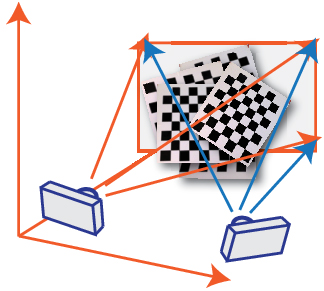
\includegraphics[width=0.6\textwidth]{figures/camCalibPosition}
		\caption[Camera-based coordinate system of MATLAB]{Camera-based coordinate system of MATLAB (\textit{source:} (\cite{StereoCalib.2016}).}
		\label{fig:camCoordinateSys}
\end{figure}

\subsubsection{Stereo Calibration Toolbox for MATLAB}\label{ssec:stereoCalibToolbox}
The \textit{Stereo Calibrator Toolbox} for MATLAB is an MATLAB application which estimates the stereo parameters of an uncalibrated stereo camera system. The toolbox was used to calibrate the two high-speed cameras in the final pipeline (\cite{StereoCalib.2016}).

\subsubsection{Camera Calibration Toolbox for MATLAB}
The \textit{Camera Calibration Toolbox} for MATLAB is another popolar alternative to calibrate a camera system. It was used to evaluate the results taken from the Stereo Calibration Toolbox. It is also included in the open source computer vision library \textit{OpenCV}\index{OpenCV}. The website provides several example projects which can be used as tutorials and it includes general information about camera calibration, which makes it a good starting point for further studies (\cite{Bouguet.2015}).

\section{Experimental Architecture} \label{sec:architecture}
The final experimental architecture of the thesis (as seen in \autoref{fig:HardwareArchitecture}) includes four lights, two synchronized high-speed cameras on a camera rig with an external trigger and the two softwares \textit{TimeBench} and \textit{MATLAB} with toolboxes. 

\begin{figure}[htbp]
		\centering
		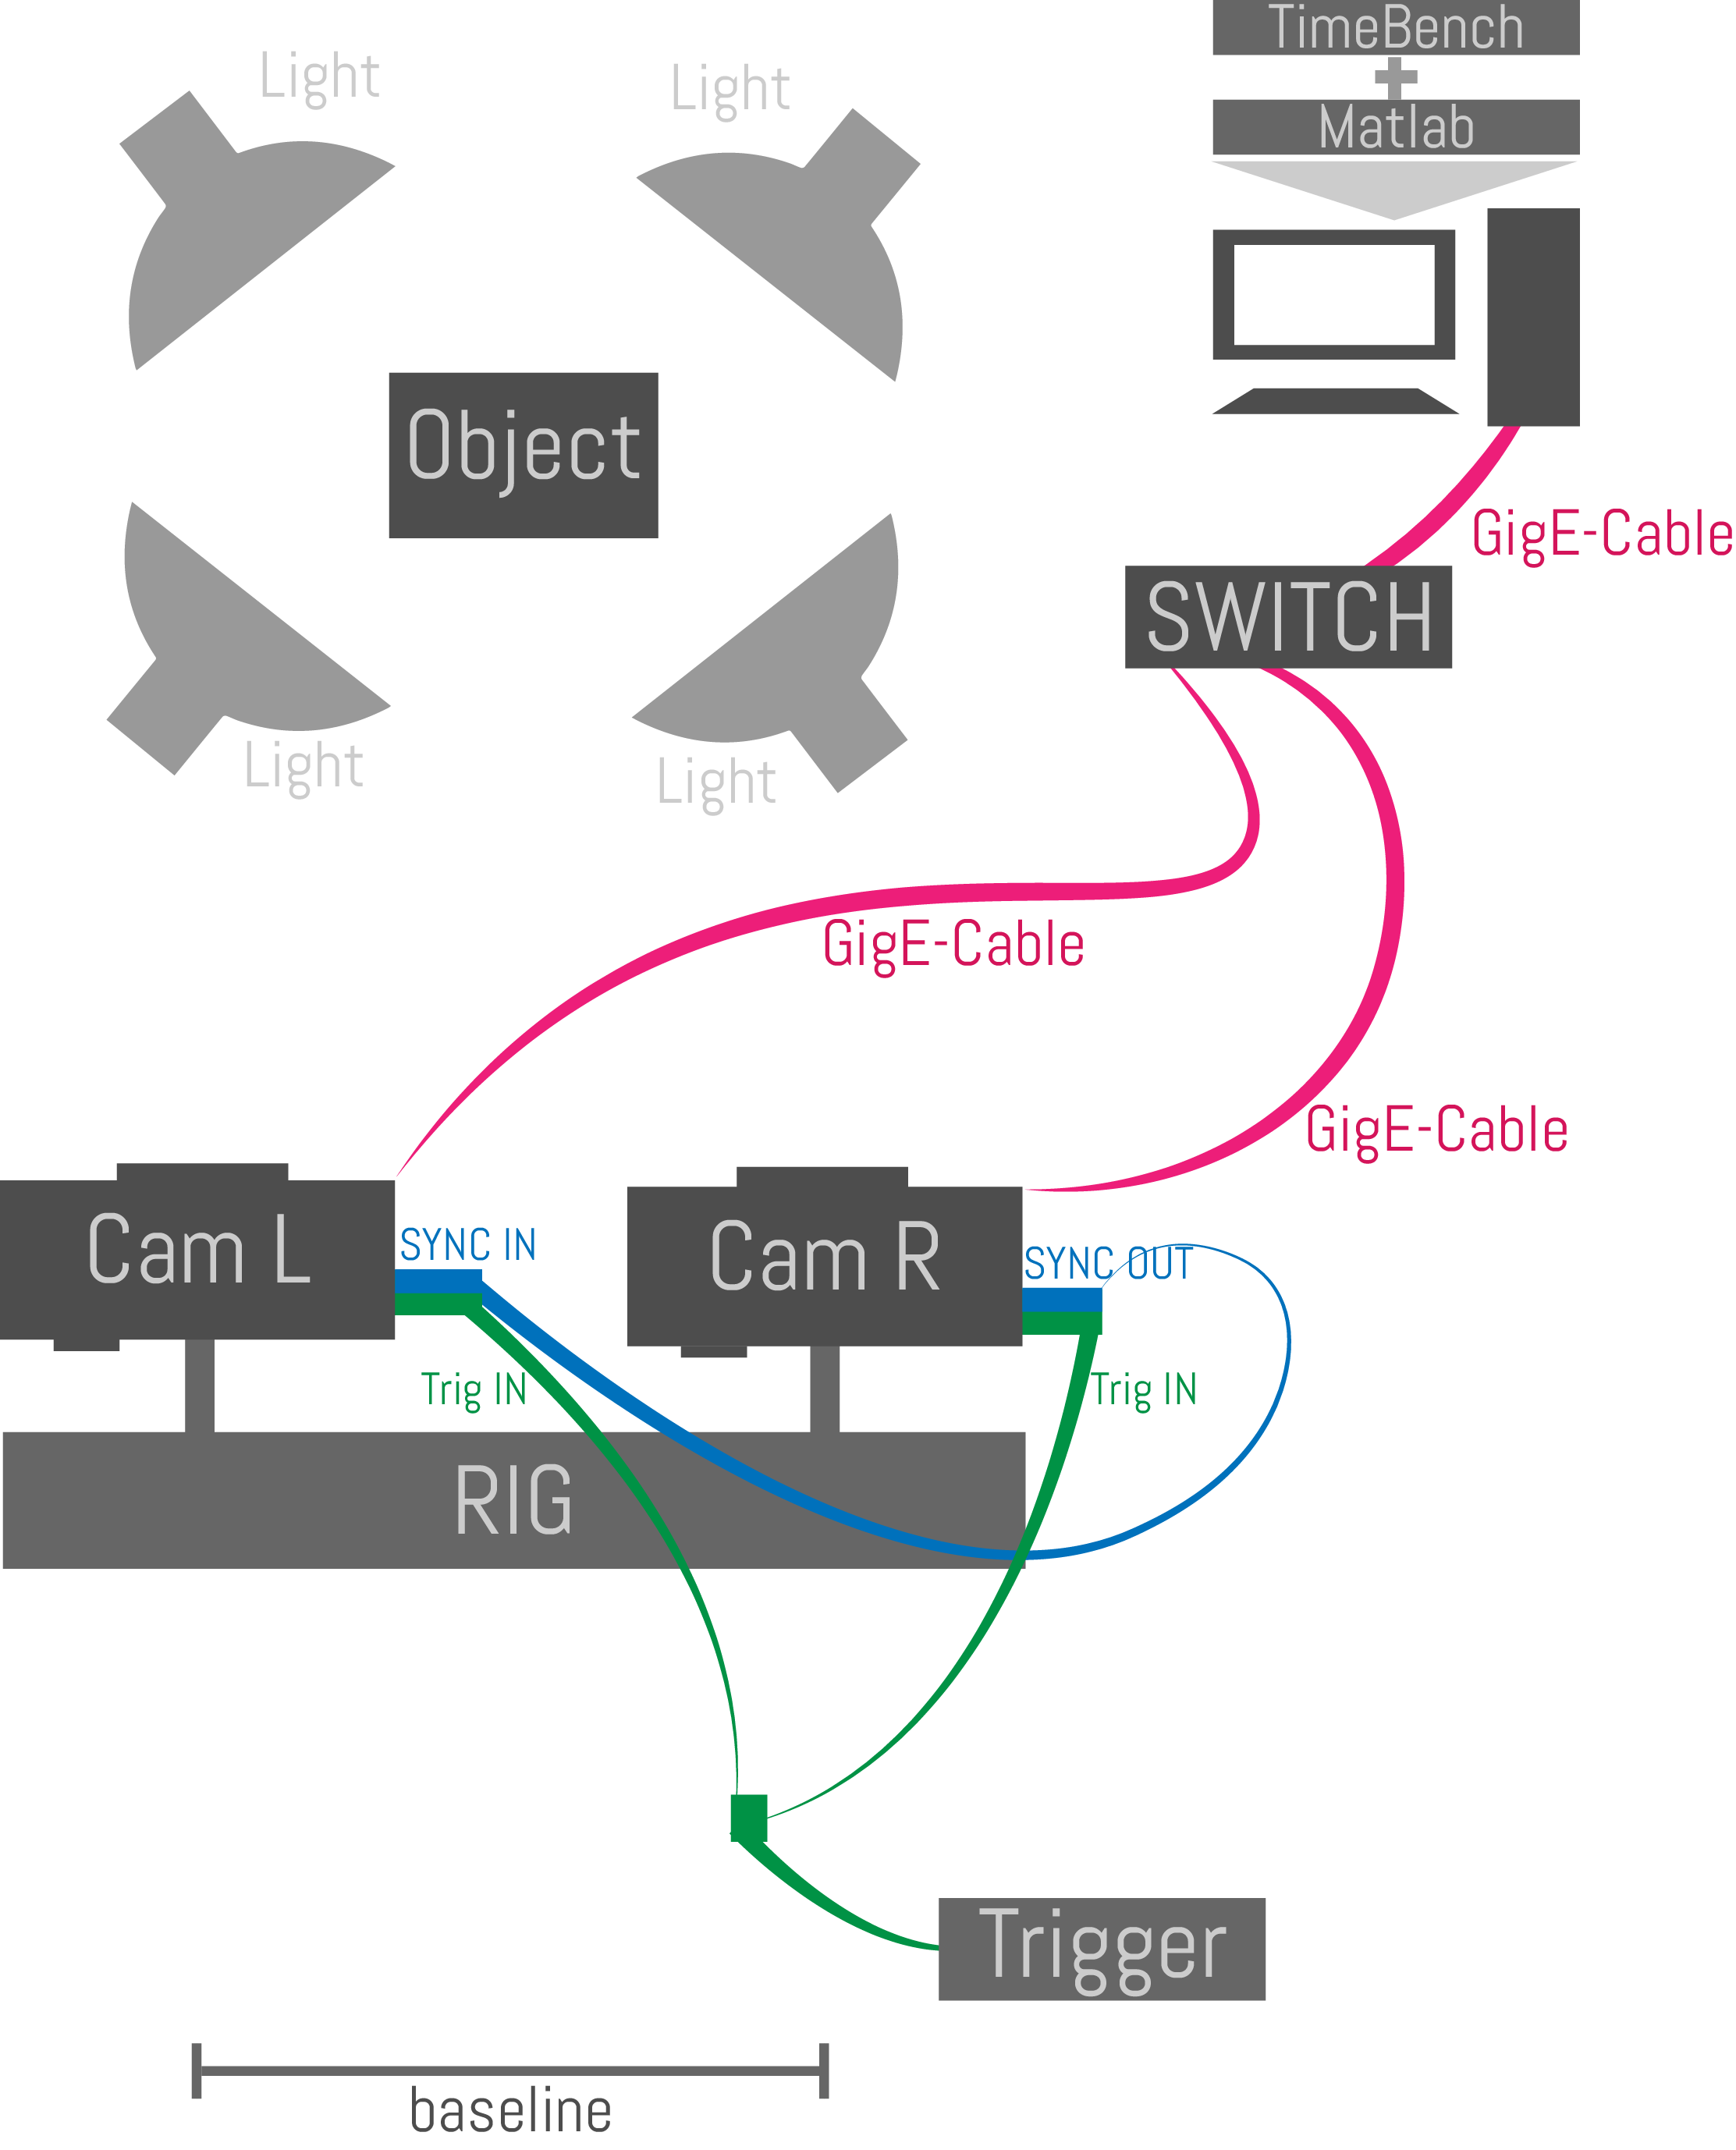
\includegraphics[width=1.0\textwidth]{figures/HardwareArchitecture}
		\caption[Hardware architecture of the final experimental set-up]{Hardware architecture of the final experimental set-up.}
		\label{fig:HardwareArchitecture}
\end{figure}